\documentclass{sig-alternate}
  %\pdfpagewidth=8.5truein
  %\pdfpageheight=11truein


%\clubpenalty=10000
%\widowpenalty = 10000

\newfont{\mycrnotice}{ptmr8t at 7pt}
\newfont{\myconfname}{ptmri8t at 7pt}
\let\crnotice\mycrnotice%
\let\confname\myconfname%


%\permission{Permission to make digital or hard copies of all or part of this work for personal or classroom use is granted without fee provided that copies are not made or distributed for profit or commercial advantage and that copies bear this notice and the full citation on the first page. Copyrights for components of this work owned by others than ACM must be honored. Abstracting with credit is permitted. To copy otherwise, or republish, to post on servers or to redistribute to lists, requires prior specific permission and/or a fee. Request permissions from permissions@acm.org.}

% --- Author Metadata here ---
\conferenceinfo{SAC'16,}{April 4-8, 2016, Pisa, Italy.}
\CopyrightYear{2016} % Allows default copyright year (2002) to be over-ridden - IF NEED BE.
\crdata{978-1-4503-3739-7/16/04...\$15.00.\\
http://dx.doi.org/xx.xxxx/xxxxxxx.xxxxxxx
}  % Allows default copyright data (X-XXXXX-XX-X/XX/XX) to be over-ridden.
% --- End of Author Metadata ---


\usepackage{cite}
\usepackage{url}
\usepackage{color}
\usepackage{listings}
\usepackage{tikz} % Need for all tikz material
\usepackage{times} % Used for formatting formatting url footnotes
\usepackage{balance}
\usepackage{framed}
\urlstyle{same} % formats footnotes
\usepackage{subfigure}
\usepackage{color,soul} % used for highlighting




\newcommand{\todo}[1]{\textcolor{cyan}{\textbf{[#1]}}}
\newcommand{\mehdi}[1]{\textcolor{red}{{\it [Mehdi says: #1]}}}
\newcommand{\dan}[1]{\textcolor{blue}{{\it [Dan says: #1]}}}


\lstset{ %
language=java,                % choose the language of the code
%xleftmargin=100pt,xrightmargin=100pt
basicstyle=\footnotesize,       % the size of the fonts that are used for the code
%numbers=left,                   % where to put the line-numbers
numberstyle=\footnotesize,      % the size of the fonts that are used for the line-numbers
stepnumber=1,                   % the step between two line-numbers. If it is 1 each line will be numbered
numbersep=3pt,                  % how far the line-numbers are from the code
backgroundcolor=\color{white},  % choose the background color. You must add \usepackage{color}
showspaces=false,               % show spaces adding particular underscores
showstringspaces=false,         % underline spaces within strings
showtabs=false,                 % show tabs within strings adding particular underscores
frame=none,           % adds a frame around the code
tabsize=2,          % sets default tabsize to 2 spaces
captionpos=t,           % sets the caption-position to bottom
%captionpos=b,           % sets the caption-position to bottom
breaklines=true,        % sets automatic line breaking
breakatwhitespace=false,    % sets if automatic breaks should only happen at whitespace
escapeinside={\%*}{*)}          % if you want to add a comment within your code
}

\setlength{\abovecaptionskip}{6pt plus 3pt minus 2pt} % Space over captions
%\setlength{\belowcaptionskip}{6pt plus 3pt minus 2pt} % Space under captions



\lstdefinestyle{ConcolicOutput}{
   % language={SQL},basicstyle=\ttfamily,
    moredelim=**[is][\btHL]{`}{`},
   % moredelim=**[is][{\btHL[fill=green!30,draw=red,dashed,thin]}]{@}{@},
}


\newif\ifisnopii
\isnopiitrue % change to true/false to remove personally identifiable information (pii)
%\isnopiifalse % change to true/false to remove personally identifiable information (pii)



%%% For adding line breaks in cells
%\newcommand{\specialcell}[2][c]{%
%  \begin{tabular}[#1]{@{}l@{}}#2\end{tabular}}



\begin{document}

% Update this title?
% An Evaluation of XXX Reverse Engineered Android Applications Through the Use of Static Analysis
\title{Architectural Clones: Toward Tactical Code Reuse}



\numberofauthors{1}
\ifisnopii % turn on/off pii
\author{
%
% 1st. author\
\alignauthor
Daniel E. Krutz and Mehdi Mirakhorl\\ 	
	\affaddr{Software Engineering Department}\\
       \affaddr{Rochester Institute of Technology}\\
       \affaddr{1 Lomb Memorial Drive}\\
       \affaddr{Rochester, NY, USA} \\
       \email{\{dkrutz, mehdi\}@se.rit.edu}
       \alignauthor
} % Must not be a space above this

\else % turn on/off pii
\author{
%
% 1st. author
\alignauthor
xxxxxxxxxxxxxxx\\ 	
	\affaddr{xxxxxxxxx}\\
       \affaddr{xxxxxxxxx}\\
       \affaddr{xxxxxxxxx}\\
       \affaddr{xxxxxxxxx, xx, xxx} \\
       \email{xxxxxx@xxxxx.xxx}
       \alignauthor
} % Must not be a space above this
\fi % end turn on/off pii

\CopyrightYear{2016} 
\setcopyright{acmcopyright}
\conferenceinfo{SAC 2016,}{April 04-08, 2016, Pisa, Italy}
\isbn{978-1-4503-3739-7/16/04}\acmPrice{\$15.00}
\doi{http://dx.doi.org/10.1145/2851613.2851787}

\maketitle

\begin{abstract}
Architectural tactics are the building blocks of software architecture. They describe solutions for addressing specific quality concerns, and are prevalent across many software systems. Once a decision is made to utilize a tactic, the developer must generate a concrete plan for implementing the tactic in the code. Unfortunately, this is a non-trivial task for even experienced developers. Developers often resort to using search engines, crowd-sourcing websites, or discussion forums to find sample code snippets. A robust Tactic Search Engine can replace this manual, internet-based search process and help developers to reuse proper architectural knowledge and accurately implement tactics and patterns from a wide range of open source systems. In this paper we analyze several implementations of architectural tactics in the open source community and identify the foundation for building a practical Tactic Search Engine. We also introduce the concept of~\emph{tactical-clones} which may be used as the basic element of a tactic search engine.


%While this paper does not present the precise details of a tactical search engine, it importantly discusses the challenges, and proposes the basis of such search engine. \dan{Maybe we should remove this last sentence? I think it removes some importance from the paper}


\end{abstract}


%% Categories taken from: http://www.jucs.org/ujs/jucs/links/Articles%20by%20Category/D.?mode=bc


%% If space is an issue, we can remove this from the 1st submission of the paper
%% We could also remove the "ermission to make digital or hard copies ....." section

%%% Check on these
\category{D.2.11}{Software Engineering} Software Architectures
\keywords{Tactical Code Clone, Software Architecture, Code Reuse}

\section{Introduction}
The success of any complex software-intensive system is dependent on how effectively it addresses the stakeholder's quality attribute concerns such as security, usability, availability, and interoperability. Designing a system to satisfy these concerns involves devising and comparing alternate solutions, understanding their trade-offs, and ultimately making a series of design choices. These architectural decisions typically begin with design primitives such as architectural tactics and patterns.

Tactics are the building blocks of architectural design~\cite{bass:arch12}, reflecting the fundamental choices that an architect makes to address a quality attribute concern. Architectural tactics come in many different shapes and sizes and describe solutions for a wide range of quality concerns. Architectural tactics are particularly prevalent across high-performance and fault tolerant software systems. Reliability tactics such as Redundancy with Voting, Heartbeat, and Check-Pointing provide solutions for fault mitigation, detection, and recovery. Performance tactics such as Resource Pooling and Scheduling help optimize response time and latency.


%% When the paper gets accepted, change the wording to no long refer to ourselves in the 3rd person

%%% Build up the previous study and show how important/profound it was. This will make our work seem more important

%%%The importance of rigorously and robustly implementing architectural tactics was highlighted by a small study conducted in an important previous work which investigated tactic implementations in Hadoop and OFBiz and evaluated their degree of stability during the maintenance process~\cite{MSRBuble}.



The importance of rigorously and robustly implementing architectural tactics was highlighted by a previous work~\cite{MSRBuble} which investigated tactic implementations in Hadoop and OFBiz and evaluated their degree of stability during the maintenance process. For each of these projects, we retrieved a list of bug fixes from the change logs (Nov. 2008 - Nov. 2011 for Hadoop, and Jan. 2009 - Nov. 2011 for OFBiz). The previous analysis showed that tactic-related classes incurred 2.8 times as many bugs in Hadoop, and 2.0 times as many bugs in OFBiz as non-tactic related classes. These observations suggest that tactic implementations, if not correctly developed, are likely to contribute towards the well-documented problem of architectural degradation~\cite{Erosion}. Less experienced developers sometimes find this challenging, primarily due to the variability points that exist in a tactic, and the numerous design decisions that need to be made in order to implement a tactic in a robust and effective way. A robust tactic search engine which can share sample code snippets from successful implementations of tactics in the open source community can be invaluable for developers.

% We found many examples of such questions in coding forums.

%A robust tactic search engine which shares sample code snippets from successful implementations of tactics in the open source community can provide valuable support for the developers.


%\begin{figure}[tbph]
%\centering
%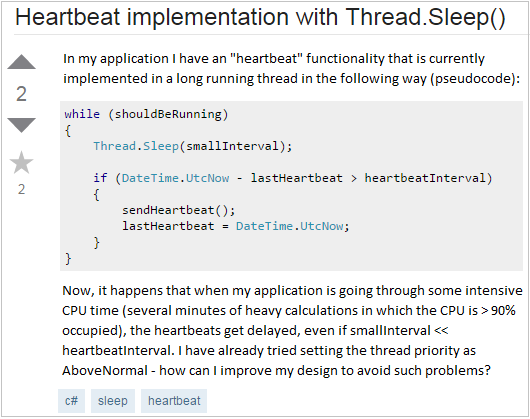
\includegraphics[width=0.99\linewidth]{./img/Question}
%\caption{}
%\label{fig:Question}
%\end{figure}




%%%% DK: I removed this to protect blind review 9/19/15
% In a previous paper we presented the overall architecture of such search engine~\cite{BIGSE}.

Our primary contributions in this paper are:
%% DK: I put these into a list since I thought it would make it really clear what our contributions were and make them easy to read

\begin{enumerate}
   \setlength{\itemsep}{0pt} %Cut down on spacing for the different items in the list
   \setlength{\parskip}{0pt} %Cut down on spacing for the different items in the list
   \setlength{\parsep}{0pt}  %Cut down on spacing for the different items in the list

  \item Report the \textit{results of a qualitative code review study} conducted to identify challenges in implementing architectural tactics and \textit{reusing tactical code}.
  \item Identify the foundations of a practical tactic search engine.
  \item Introduce the notion of \textit{tactical clones} and formulate the next steps in realizing a tactic search engine.
\end{enumerate}


%A) Reporting the \textit{results of a qualitative code review study} conducted to identify challenges in implementing architectural tactics and \textit{reusing tactical code}. B) Identifying the foundations of a practical tactic search engine. C) Introducing the notion of \textit{tactical clones} and formulating the next steps in realizing tactic search engine.

Although there has been some initial development of source code recommender systems~\cite{DBLP:conf/icse/McMillanHPCM12,6340250}, the primary focus of this previous research is only on retrieving generic functional code and not tactical code. Therefore the challenges of obtaining and recommending tactical code is still unexplored. This paper focuses on identifying these challenges.

This paper organized as follows: Section~\ref{sec:Method} presents the underlying methodology used to conduct the qualitative study of tactic implementations. Section \ref{sec:SeenUnSeen} discusses the results of our qualitative study, tactic implementation issues, reusability concerns and other observations across several implementation of architectural tactics. This section also summarizes the foundations for developing a practical tactic search engine. Section \ref{sec:Clones} presents the definitions of tactical clones and the process of extracting sample architectural clones from source code of several open source systems. Section \ref{sec:Future} presents possible future work to build on our research and Section \ref{sec: relatedwork} discusses related works. Section \ref{sec:Conclusion} concludes our paper. 

\input{sections/SeenUnSeen.tex}
\section{Architectural Clones: A Step Toward Tactical Code Reuse}
\label{sec:Clones}
%\hl{The qualitative study conducted in this paper, motivated utilization of tactical clones as the minimum practical reuse granularity.}

The qualitative study we conducted motivated the utilization of tactical clones as an appropriate level of granularity in respect to code reusability. In order to illustrate the concepts of architectural or tactical clones, our qualitative study was followed by an exploratory study where we established a representative sample of these design clones. To assist, we developed a semi-automated process for retrieving candidate instances of tactic-related classes then detected code clones across these tactical files. 

The process of detecting tactical clones involves the following steps: (1) building a software repository, (2) extracting instances of architectural tactics, (3) extracting code clones across projects, and (4) manually inspecting the results to investigate our hypothesis that tactical clones are a practical granularity for architectural reuse.

\subsection{Building a software repository}

To build our repository of software systems, we preselected 37 open source projects with a high number of architectural tactics.

\begin{figure*}[!t]
\vspace{-1pt}
\centering
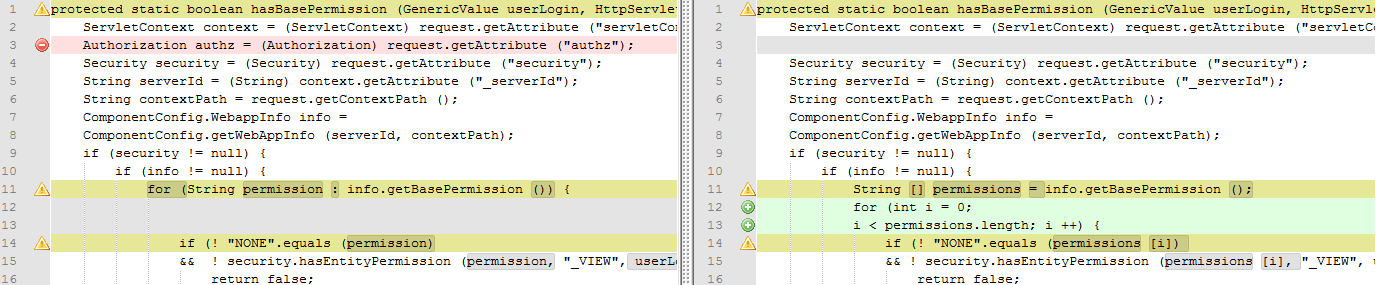
\includegraphics[width=0.9\linewidth]{./img/Permission}
\vspace{-6pt}
\caption{Tactical Clones Detected in Two different Projects}
\label{fig:Permission}
\vspace{-1pt}
\end{figure*}



\subsection{Extracting architectural tactics}
We utilized a previously developed tactic detection algorithm and tool~\cite{ICSE2012, FSE2014} to identify architectural tactics. These Tactic Detector's classifiers have been trained to find architectural tactics such as \textit{audit trail}, \textit{asynchronous method invocation}, \textit{authentication}, \textit{checkpointing and roll back}, \textit{Heartbeat}, \textit{role-based access control (RBAC)}, \textit{resource pooling}, \textit{scheduling}, \textit{ping echo}, \textit{hash-based method authentication}, \textit{kerberos} and \textit{secure session management}. Due to space constraints, we provide only an informal description of our tactic detection approach. However a more complete description of the approach, including its related formulas, may be found in previous publications~\cite{Dissertation, ICSE2012}. The tactic detection technique uses a set of classification techniques. These classifiers are trained using code snippets representing different architectural tactics, collected from hundreds of high-performance, open-source projects \cite{FSE2012,ICSE2012,Dissertation}. During the training phase, the classifier learns the terms (method and variable names as well as development APIs) that developers typically use to implement each tactic and assigns each potential indicator term a weight with respect to each type of tactic. The weight estimates how strongly an indicator term signals an architectural tactic. For instance, the term \emph{priority} is found more commonly in code related to the \emph{scheduling} tactic than in other kinds of code, and therefore the classifier assigns it a higher weighting with respect to scheduling. During the classification phase, the indicator terms are used to evaluate the likelihood that a given file implements an architectural tactic.

The accuracy of the Tactic Detector has been evaluated in several studies \cite{ICSE2012,FSE2014,Dissertation}. In a series of  experiments it was able to correctly reject approximately 77-100\% of non-tactical code classes (depending on tactic types); recall 100\% of the tactics-related classes with precision of 65\% to 100\% for most tactics tactics.  The recall for the authentication, audit trail and asynchronous method invocation was 70\% .

While this approach does not return perfectly precise results, it has a tuning parameter which enables us to only include the tactical files with higher prediction confidence in our analysis, which will significantly reduce the search space and assist with the task of retrieving candidate tactical clones.


%The final projects are listed in Table \ref{tab:ChosenProjects}. For each project we report its name, the number of classes in the system, the number of tactic types covered (maximum 13), number of candidate design patterns detected (maximum 20), and the final count of pattern/tactic overlaps as predicted by our automated tools.  As depicted in this table, most of the included projects provided coverage of 5 or more tactic types; however in order to ensure coverage of all the studied tactics, we included a couple of additional projects simply because they included the targeted tactic type, even though their overall tactic coverage was low.

%%%%%%%%%%%%%%%%%%%%%%%%%%%%%%


\subsection{Detecting Tactical Clones}
In order to detect architectural clones we used code clone detection techniques to identify reused tactical methods across different projects. We define the four types of tactical code clones by extending the definitions from Roy et al.~\cite{Roy:2008:NAD:1437898.1438600}.


\textbf{Type-1 tactical clones} are the simplest, representing identical tactical code except for variations in whitespace, comments, and layout to the type-4 clones, which are the most complex.


\textbf{Type-2 tactical clones} have variations in identifiers, types, whitespace, literals, layout, and comments, but are otherwise syntactically identical.

\textbf{Type-3 tactical clones} are tactical fragments which are copied and have modifications such as added or removed statements, variations in literals, identifiers, whitespace, layout and comments.


\textbf{Type-4 tactical clones}, are tactical code segments that perform the same computation, but have been implemented using different syntactic variants. 
%Concolic analysis ~\cite{Sen:2005:CCU:1081706.1081750} can be used to detect type-4 tactical clones~\cite{wcre2013}.


% Traditionally it has been used for software testing~\cite{Sen:2005:CCU:1081706.1081750}, code clone detection~\cite{wcre2013}, and vulnerability recognition~\cite{Chen:2014:CIB:2554850.2554875}.


In an extensive experiment we ran a leading clone detection tool Nicad~\cite{Roy:2008:NAD:1437898.1438600}, over the tactical code snippets from 37 projects. We chose Nicad for our analysis since it is a mature and refined tool which has demonstrated its effectiveness in previous research~\cite{roy2008empirical}.

\begin{table}[tbph]
\vspace{-10pt}
\caption{Discovered Tactical Clones Across 37 Projects.}
\label{tab:ChosenProjects}
\centering

%\begin{tabular}{|p{2.0cm}|p{2cm}|p{2.4cm}|}
  \begin{tabular}{ c | l | l }
\hline

\bfseries Tactic & \bfseries Number~of~Clones & \bfseries In~Total~Tactical~Files \\ \hline \hline
Audit & 50    & 352 \\ \hline
Authenticate & 151   & 252 \\\hline
Checkpointing & 8     & 138 \\ \hline
Ping Echo & 10    & 103 \\ \hline
Pooling & 1021  & 1073 \\ \hline
RBAC  & 436   & 477 \\ \hline
Scheduling & 76    & 117 \\ \hline
Secure Session & 249   & 299 \\ \hline
HeartBeat & 0     & 11 \\ \hline
Kerbrose & 0     & 21 \\
\end{tabular}%
\vspace{-10pt}
\end{table}

\subsection{Results}
Table~\ref{tab:ChosenProjects} shows tactics used in our study, as well as the number of tactical clones across projects. The last column of this table illustrates the total number of tactical files used in our analysis. The tactical clones were detected at the method level. While we could have detected tactical clones at the sub-method level, we realized that method level tactical clones are easier to comprehend and therefore easier to reuse for the developers. We do not report tactical clones within the same project since developers typically reuse the source code within a project. We were interested in the tactical clones reused across various projects so we could identify intrinsic and reusable tactical code snippets. As a result of our exploratory study we found several examples of identical tactical code snippets. While most of the clones were type 1, 2 and 3, we also had several examples of \textit{conceptually equivalent} tactical code snippets (type 4).

 Figure~\ref{fig:Permission} shows the source code for RBAC tactics across two different projects. In this example two developers in different systems have potentially created the same code snippets to implement the tactic. This example is one instance among several similar observations of tactical clones across different projects. This supports the hypothesis that tactical clones are an appropriate level of granularity in respect to code reusability. However, as stated in future work we plan to examine this hypothesis in set of developer studies.


%  This observation and several similar detected clones also support the hypothesis the fact that tactical clones are a more common granularity for code adoption and reuse.



\noindent
\vspace{-2pt}
\begin{table*}[ht]
\caption{An Example HeartBeat Tactical Clone~\label{table:heartbeedexample}}
\centering
\begin{tabular}{c | c}
\bfseries HeartBeat Example \#1  & \bfseries HeartBeat Example \#2  \\ \hline \hline
\begin{lstlisting}
boolean shouldBeRunning=true;
int smallInterval=10;
long lastHeartbeat=0;
int heartbeatInterval=10;
while (shouldBeRunning){
  Thread.sleep(smallInterval);
  if(System.currentTimeMillis()-lastHeartbeat>
    heartbeatInterval){
    sendHeartbeat();
    lastHeartbeat= System.currentTimeMillis();
  }
}
\end{lstlisting}
&
\begin{lstlisting}
long lastRunTime=0; 
long timeSpan=System.currentTimeMillis();
long timeSinceLastRun=
  System.currentTimeMillis()-lastRunTime;
  if(timeSinceLastRun>10) {
    sendHeartbeat();
  lastRunTime = System.currentTimeMillis();
}
\end{lstlisting} 
\end{tabular}
\vspace{-2pt}
\end{table*}


\vspace{-10pt}
\section{Future Work}
\label{sec:Future}
This paper provides crucial information about tactic implementation and code reuse. However, there is still future work to be conducted in this area.

\subsection{Conceptually Equivalent Tactical Clones}
While tactical clone types 1, 2, and 3 primarily represent syntactically equivalent tactical code snippets reused across various projects, sharing and reusing tactical code snippets that are type 4 clones would be very beneficial. Our initial investigation indicates that type-4 or semantically equivalent tactical clones can be detected using complex code similarity techniques such as symbolic and concolic analysis~\cite{wcre2013, Dan123}.

Concolic analysis combines concrete and symbolic values to traverse all possible paths of an application. Since concolic analysis is not affected by syntax or comments, identically traversed paths are indications of duplicate functionality, and therefore functionally equivalent code. These traversed paths are expressed in the form of~\emph{concolic output} which represents the execution path tree and displays the utilized path conditions and representative input variables. In order to detect tactical-clones we used a concolic analysis based clone detection technique \cite{wcre2013,Dan123, Krutz:2015:EEU:2695664.2695929} on two type-4 clone examples examples of Heartbeat are shown in Table~\ref{table:heartbeedexample}.

We then ran concolic analysis on these two code segments which produced the matching concolic output shown in Table~\ref{fig:exampleoutput} which indicated that original code snippets are tactical type-4 clones. In this example, variable type integers are represented by a generic tag ``SYMINT.'' Though not present in this example, other variable types are represented in a similar fashion in concolic output. Actual variable names do not appear anywhere in the output and are irrelevant to this clone detection process. This can be very beneficial for the type-4 clone detection process. We anticipate that open source repositories have a large number of tactical type-4 clones which can be used as input for a tactic search engine.

In future work we plan to extend a primitive clone detection technique based on concolic analysis that is able to identify semantically equivalent code snippets. We will also augment this approach with text mining and information retrieval techniques.

\subsection{Large Scale Study}
Future work should also include a larger scale study where at least several hundred open source projects will be studied to better understand how pervasive tactical clones are. We will also conduct a quantitative study to compliment our initial qualitative study reported in this paper. For each of the identified issues, we will examine how frequently they occur across different implementations of tactics.


\subsection{Developer Study}
A series of experiments are required to rigorously evaluate the practical value of tactical clones in software reusability. A study may be conducted where developers can use a tactic-search engine to look for tactic implementations in terms of clones. The developer feedback regarding the usefulness, reusability and practicality of retrieved tactical code would then be collected.

 
%% Use different clone detection tools & techniques such as Simian\footnote{\url{http://www.redhillconsulting.com.au/products/simian/}}, CloneDR\footnote{\url{http://www.semdesigns.com/products/clone/}}, MeCC\footnote{\url{http://ropas.snu.ac.kr/mecc/}}, CCCD~\cite{Krutz:2015:EEU:2695664.2695929}, and Simcad~\cite{6613857}



\noindent
\begin{table}[hb] %h for here, t for top, b for bottom
\vspace{-16pt}
\caption{Diff of HeartBeat Concolic Output}
~\label{table:concolicoutputcomparision}
\centering
\begin{tabular}{ p{3.8cm} | p{3.8cm} }
\multicolumn{1}{c}{\textbf{Concolic Segment \#1}} & \multicolumn{1}{c}{\textbf{Concolic Segment \#2}} \\ \hline \hline
\begin{lstlisting}[style=ConcolicOutput]
### PCs: 1 1 0
a_1_SYMINT,
a_1_SYMINT,d1_2_SYMREAL,
a_1_SYMINT,d1_2_SYMREAL,s1_3_SYMSTRING,
\end{lstlisting}
&
\begin{lstlisting}[style=ConcolicOutput]
### PCs: 1 1 0
a_1_SYMINT,
a_1_SYMINT,d1_2_SYMREAL,
a_1_SYMINT,d1_2_SYMREAL,s1_3_SYMSTRING,
\end{lstlisting}

\end{tabular}
\label{fig:exampleoutput}
\vspace{-10pt}
\end{table}


Several other works have discussed the importance of design in agile software development. Wirfs-Brock~\cite{Wirfs-Brock:2010:SAD:1869542.1869630} spoke about the significance of agile developers having the ability to quickly understand design problems and make timely decisions about how to address the issue. 

While our work is innovative, there are a wide range of existing techniques that support agile software development. Spoelstra et al.\cite{Spoelstra:2011:SRA:1982185.1982255} proposed a conceptual management tool for supporting software reuse in agile software development using a components derived from the Software Process Improvement (SPI) framework by Niazi et al.\cite{Niazi:2005:MMI:1045926.1045932}. Their tool utilizes maturity levels and reuse practices in order to create a reuse maturity model. However, none were specifically focused on agile architecture development. There is a wide range of other tools supporting agile software development including tools for software project management and planning~\cite{Petersen:2008:APT:1379092.1379101, Dhlamini:2009:IRM:1562741.1562745}, and modeling~\cite{Buchmann:2012:TTS:2467307.2467310}. 

Several researchers have attempted to address architectural challenges through developing techniques for organizing, documenting or modeling architectural decisions. The Architecture Design Decision Support System (ADDSS)\cite{ADDSS}, Process based Architecture Knowledge Management Environment (PAKME)\cite{PAKME}, and Architecture Rationale and Element Linkage (AREL)\cite{AREL} are examples of these. However, these approaches are not adopted to the agile development mindset, and fail to address the scalability issues of managing potentially large numbers of architectural decisions.  They also fail to connect design decisions to code, and/or provide little support for actually utilizing this knowledge during software maintenance. 





\section{Conclusion}
\label{sec:Conclusion}
In this work we investigated the challenges toward creating a robust and practical tactic search engine. The study revealed issues related to coding architectural tactics. Furthermore, our study suggests that the notion of architectural clones can provide a reusable level of granularity for a tactic search engine. Future work will examine this suggestion through a rigorous developer study.

\section{Acknowledgments}
The work in this paper was partially funded by the US
National Science Foundation grant \#CCF-1543176. 


\balance
\bibliographystyle{abbrv}
\bibliography{architecturalclones}



% That's all folks!
\end{document}


% Submission information
%   Confirmation Number: 1695
%   Submission Passcode: 1695X-F9J6A2A7A4
%   https://www.softconf.com/f/sac2016/cgi-bin/scmd.cgi?scmd=aLogin&passcode=1695X-F9J6A2A7A4





%%%
%? Tactic or tactical ? --
% X  heartbeat or Heartbeat
%   should architectural tactics be capitalized ?
%   tactical-clones or tactical clones
%   make sure that everything is actually anonymous

%%%
% - Remove all "red" misspelling
% - Work on formatting
% - data set, or dataset
% - search for ?


%%%% Reviews
%   Clarify much of the work
%   Make it "bold"




